\section{Ontology}
Choose Well defines its own RDF vocabulary. 
% \todo[inline]{Later - add figure number}
Fig. x contains the ontology as a UML class diagram. 
The diagram uses these prefixes:
% \todo[inline]{After exams - change font of prefixes to code}
% \todo[inline]{After exams - add arrow symbols for prefixes}
% \todo[inline]{After exams - look for a nicer hash symbol}

\begin{itemize}[noitemsep,nolistsep]
  \item cw: \textbf{https://github.com/JiriResler/solid-choose-well-ontology/} \newline \textbf{blob/main/choosewell\#} for the Choose Well ontology.
  \item schema: \textbf{http://schema.org/} for the Schema.org general vocabulary. 
  \item rdfs: \textbf{http://www.w3.org/2000/01/rdf-schema\#} for the RDF Schema which provides a data-modelling vocabulary for RDF data.
  \item wikidata: \textbf{http://www.wikidata.org/entity/} for describing entities using the Wikidata knowledge base.
\end{itemize}

\begin{figure}[h]
  \centering
  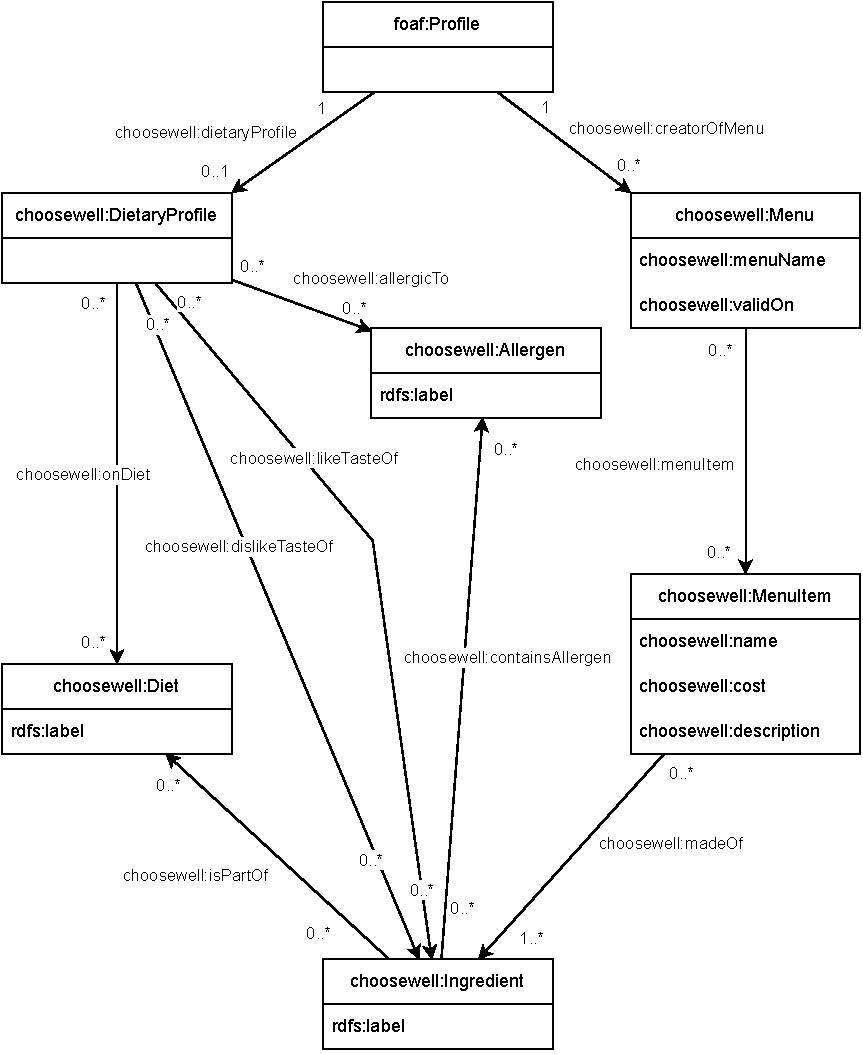
\includegraphics[width=\linewidth]{master-thesis/img/design-ontology.pdf}
  \caption{The Choose Well ontology}
\end{figure}
